\section*{引言}

本文档，整理总结了使用边界层理论、势流理论分析贴附通风气流组织问题的过程以及相关的推导细节。

\subsection{坐标系以及物理描述}
为了方便分析不同区域的流动，建立两个坐标系。

第一个坐标系原点位于房间左下角，$x$为水平方向，$y$为竖直向上方向，假设房间层高为$H$。

第二个坐标系原点位于房间左上角，$x$仍为水平方向，$y'$为竖直向下方向，竖直方向的坐标满足$y=H-y'$

送风口位于$y=H(y'=0)$的房间顶部，宽度为$B$，风口中心位于$x=x_{c}$，送风速度均匀向下，表示为$U_{0}$。
\begin{figure}[htb]
	\centering
	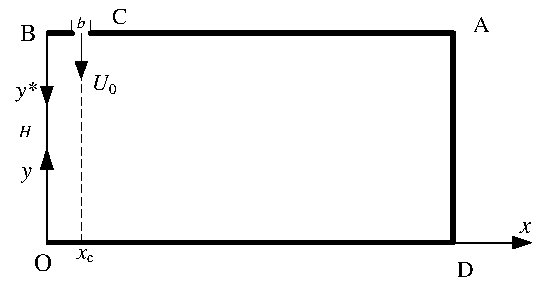
\includegraphics[width=\linewidth]{figs/zuobiaoxi.pdf}
	\caption{坐标系定义}
	\label{zuobiaoxi}
\end{figure}



